%!TEX program = pdflatex
\documentclass[11pt,a4paper]{article}

\usepackage[margin=1in]{geometry}
\usepackage{amsmath}
\usepackage{booktabs}
\usepackage{graphicx}
\usepackage{hyperref}
\usepackage{threeparttable}

% Figures live under results/ relative to this file (docs/)
\graphicspath{{../results/person2/figures/}}

\hypersetup{
  colorlinks=true,
  linkcolor=blue,
  urlcolor=blue,
  pdftitle={Chunking and Top-k Retrieval Ablations for Guideline RAG}
}

\title{Chunking Strategy and Top-\(k\) Retrieval Ablations\\
  for Dense Retrieval-Augmented Generation on Clinical Guidelines}

\author{\textbf{[Author / Group — Person 2]}\\
  ICS4554 Natural Language Processing / AfriMed Tutor}
\date{\today}

\begin{document}
\maketitle

\begin{abstract}
We report three controlled ablations for a dense retrieval-augmented generation (RAG) system over a multi-document PDF guideline corpus, evaluated on a stratified held-out set of 100 multiple-choice items from AfriMed-QA. Experiments compare (E1) structure-aware segmentation versus a naive sliding-window baseline, (E2) four nominal maximum chunk lengths under the structure-aware policy, and (E3) retrieval depth \(k \in \{1,3,5,10,15\}\) holding the index fixed. MCQ accuracy varied only within a narrow band (point estimates 0.63--0.66); bootstrap \(95\%\) confidence intervals overlapped across most conditions. Structure-aware and naive chunking did not differ significantly by an exact McNemar test on paired correctness (\(p = 0.625\)). Increasing \(k\) yielded no clear monotonic accuracy gain; billed input length to the generator was nearly flat across \(k\), consistent with similarity-based filtering capping the number of passages actually injected into the prompt regardless of nominal top-\(k\). We interpret these patterns as evidence of a \emph{weak local sensitivity} of this pipeline to the swept hyperparameters under the chosen model, threshold, and finite test sample, and we stress limitations of \(n=100\) and a single decoder backbone.
\end{abstract}

\section{Introduction}
Long-form clinical guidelines are semi-structured texts: sections, bullets, and enumerated protocols co-exist with heterogeneous layout. Retrieval-augmented generation typically segments documents into passages that are independently embedded and retrieved. \emph{Structure-aware} segmentation aims to honor natural boundaries (sections, paragraphs) before applying length limits, whereas \emph{naive} sliding windows ignore document structure. One expects structure-aware chunking to yield more coherent retrieval units and, downstream, better task performance when answers depend on localized protocol blocks~\cite{ragplaceholder}. The empirical question is whether these differences materialize as measurable gains on a fixed multiple-choice benchmark under a fixed decoder and embedding family.

A second axis is \emph{passage budget}: retrieving more candidates may improve recall of the supporting passage, but can also inject noise and increase latency and cost~\cite{longcontextplaceholder}. We therefore sweep nominal top-\(k\) while holding the vector index fixed.

This note synthesizes completed ablations E1--E3 using a single dense retriever, a single embedding model family, and held-out AfriMed-QA items, with statistics appropriate to paired and unpaired binary outcomes.

\section{Materials and methods}

\subsection{Guideline corpus}
The retrieval corpus consists of licensed or publicly available national and international clinical guideline PDFs spanning primary care, hospital care, and maternal/child exemplars (Southern Africa, West Africa, Kenya, and WHO sources). Text was extracted programmatically from PDFs (with the usual caveat that complex tables and figure-heavy pages may be imperfectly represented). Each experimental condition produced a distinct chunked representation and a separate dense vector index; no cross-mixing of chunk sets between conditions.

\subsection{Segmentation conditions}
\textbf{(E1 --- structure vs.\ naive.)} The \emph{structure-aware} pipeline first segments on detected section headings (pattern families tuned to each document source), then subdivides oversized sections at paragraph boundaries subject to a nominal maximum length in \emph{approximately} tokenized units (heuristic word-length scaling) with bounded overlap between adjacent pieces. The condition used for the structured baseline in E1 matched an 800-unit ceiling used elsewhere in the project. The \emph{naive} baseline applied a fixed character window of 800 characters with stride determined by a 200-character overlap, without inferred section metadata, matching a standard ``no structure'' RAG baseline.

\textbf{(E2 --- chunk-size ablation.)} Under the structure-aware policy only, nominal maximum segment lengths were set to \(\{100,\,200,\,400,\,800\}\) in the same approximate token units, holding overlap and heading rules fixed. Empirically, corpus-level mean token or word statistics and index cardinalities moved only slightly across these settings because many natural sections already fell under the ceiling.

\subsection{Embeddings and indexing}
Passage embeddings were computed with a commercial small-dimensional dense embedding model (\textbf{[fill: e.g.\ OpenAI \texttt{text-embedding-3-small}]}). A tokenizer-based hard ceiling (8192-token class limit for the provider; internal budget set below that) was applied \emph{before} embedding call batches so that pathological PDF spans with few whitespace breaks could not violate API limits. Rare segments were split into multiple index rows. Vectors were \(\ell_2\)-normalized; retrieval used inner product as a cosine similarity surrogate on the unit sphere.

\subsection{Dense retrieval and \texorpdfstring{top-\(k\)}{top-k} sweep}
Retrieval was purely dense (no sparse fusion in these runs). The \(k\) nearest passages by similarity were considered, but passages scoring below a fixed \textbf{minimum similarity threshold} \textbf{[\(\tau\) --- fill from configuration, e.g.\ 0.30]} were discarded. \textbf{(E3)} used the highest-accuracy index configuration from E2 under the project's selection rule (tie-break: lower mean end-to-end latency when accuracies matched). Nominal \(k \in \{1,3,5,10,15\}\) was varied; the decoder prompt included all retained passages (with source tags) up to the truncated list.

\subsection{Generation and decoding}
A single instruction-tuned causal language model (\textbf{[fill: provider and model identifier]}) answered each multiple-choice item. The prompt required the model to output only the letter of the chosen option. Decoding used \textbf{[fill: temperature, default 0 if applicable]}. No chain-of-thought or explanation was elicited during scoring.

\subsection{Evaluation set and metrics}
Evaluation used a held-out stratified sample of \textbf{100} AfriMed-QA multiple-choice questions, \textbf{twenty} items from each of five clinical groupings (Surgery; Obstetrics \& Gynecology; Pediatrics; Infectious Disease; Internal Medicine). Accuracy is the fraction of items whose predicted letter exactly matches the keyed answer. For each condition, \textbf{bootstrap \(95\%\) confidence intervals} for accuracy were formed by resampling the 100 items with replacement \textbf{(4{,}000 replicates; seed fixed for reproducibility)}. For E1, paired outcomes were compared with an \textbf{exact two-sided McNemar} binomial test on discordant pairs.

Auxiliary logged quantities (mean billed input tokens per item, mean first-passage similarity, wall-clock latency per item) are reported descriptively without inferential claims.

\subsection{Reproducibility}
An experiment manifest records software context (e.g.\ git revision \texttt{0da454a}, Python 3.10.19, timestamp 2026-05-01Z) and the policy of holding the test split, embedding provider, dense backend, and decoding policy fixed across conditions except where explicitly ablated.

% --- Bibliography: replace with bibtex file or full entries ---
\begin{thebibliography}{9}
  \bibitem{ragplaceholder} Lewis, P.\ et al.\ (2020). Retrieval-augmented generation for NLP tasks. (\emph{Citation stub --- replace}.)
  \bibitem{longcontextplaceholder} Surveys on long-context and noise in retrieval-augmented LMs (\emph{Citation stub --- replace}.)
\end{thebibliography}

\section{Results}

\subsection*{E2: nominal maximum chunk length (structure-aware only)}
Across \(\{100,200,400,800\}\), MCQ accuracy was \textbf{0.63} for every bucket. Bootstrap \(95\%\) intervals were overlapping (approximately 0.53--0.72). Chunk inventory statistics drifted mildly (e.g.\ indexed segments \(5648\)--\(5656\); mean word length \(\approx 144\)), consistent with segmentation being governed primarily by headings and paragraphs rather than the nominal ceiling across this grid.

\subsection*{E1: structure-aware versus naive sliding window}
Structure-aware indexing achieved accuracy \textbf{0.64} (bootstrap interval approximately 0.54--0.73); naive windows achieved \textbf{0.66} (approximately 0.57--0.75). Discordant pairwise outcomes numbered \textbf{four} exclusively: \textbf{three} cases where structure-aware answered incorrectly while naive succeeded, versus \textbf{one} reciprocal case (\(p = 0.625\) McNemar exact two-sided test). Interpretation-wise, we \emph{cannot reject} parity; the directional advantage of naive segmentation in held-out accuracy is statistically weak and hypothesis-inconsistent.

\subsection*{E3: nominal top-\(k\)}
Accuracy remained at \textbf{0.63} for \(k \in \{1,3,5,15\}\) and rose to \textbf{0.64} for \(k = 10\), inside overlapping bootstrap bands. Mean billed prompt length stayed near \textbf{2002 tokens} regardless of nominal \(k\), suggesting the similarity floor \textbf{already limited} how many excerpts cleared the retrieval filter across this benchmark. Mean wall-clock latency for \(k=1\) exhibited a higher mean (\(\approx 2475~\mathrm{ms}\)) and dispersion than \(k \geq 3\); speculative drivers include provider jitter or heterogeneous item difficulty but were not isolated here.

\section{Tables and figures}

\begin{table}[t]
  \centering
  \begin{threeparttable}
    \caption{E2 --- MCQ accuracy and approximate \(95\%\) bootstrap intervals (\(n=100\)).}
    \label{tab:e2}
    \begin{tabular}{lccc}
      \toprule
      Nominal max.\ chunk length & Accuracy & \(95\%\) CI low & \(95\%\) CI high \\
      \midrule
      100 & 0.63 & 0.53 & 0.72 \\
      200 & 0.63 & 0.53 & 0.72 \\
      400 & 0.63 & 0.53 & 0.72 \\
      800 & 0.63 & 0.53 & 0.72 \\
      \bottomrule
    \end{tabular}
  \end{threeparttable}
\end{table}

\begin{table}[t]
  \centering
  \begin{threeparttable}
    \caption{Corpus fragmentation under E2 / E1 structured conditions (indexed segments before query-time retrieval). Naive corpus is structurally incomparable.}
    \label{tab:chunks}
    \begin{tabular}{lccc}
      \toprule
      Condition & Indexed segments & Mean words / segment & Median words \\
      \midrule
      E2 (100) & 5656 & 144.16 & 71 \\
      E2 (200) & 5654 & 144.21 & 71 \\
      E2 (400) & 5648 & 144.36 & 71 \\
      E2 (800) & 5635 & 144.68 & 71 \\
      E1 structure & 5635 & 144.68 & 71 \\
      E1 naive & 9765 & 113.56 & 115 \\
      \bottomrule
    \end{tabular}
  \end{threeparttable}
\end{table}

\begin{table}[t]
  \centering
  \begin{threeparttable}
    \caption{E1 --- pairwise comparison (paired items, \(n{=}100\) each). Discordant counts are exact McNemar input.}
    \label{tab:e1}
    \begin{tabular}{lc}
      \toprule
      Metric & Value \\
      \midrule
      Structure-aware accuracy & 0.64 \\
      Naive accuracy & 0.66 \\
      Discordant pairs (structured wrong \(\land\) naive correct) \(b\) & 3 \\
      Discordant pairs (structured correct \(\land\) naive wrong) \(c\) & 1 \\
      McNemar \(p\)-value (two-sided exact) & 0.625 \\
      \bottomrule
    \end{tabular}
  \end{threeparttable}
\end{table}

\begin{table}[t]
  \centering
  \begin{threeparttable}
    \caption{E3 --- MCQ accuracy, mean billed input tokens, and latency.}
    \label{tab:e3}
    \begin{tabular}{cccc}
      \toprule
      \(k\) & Accuracy & Mean input tokens & Mean latency (ms) \\
      \midrule
      1  & 0.63 & 2002.7 & 2475 \\
      3  & 0.63 & 2002.7 & 1848 \\
      5  & 0.63 & 2002.7 & 1928 \\
      10 & 0.64 & 2002.7 & 1821 \\
      15 & 0.63 & 2002.7 & 1833 \\
      \bottomrule
    \end{tabular}
  \end{threeparttable}
\end{table}

\begin{figure}[t]
  \centering
  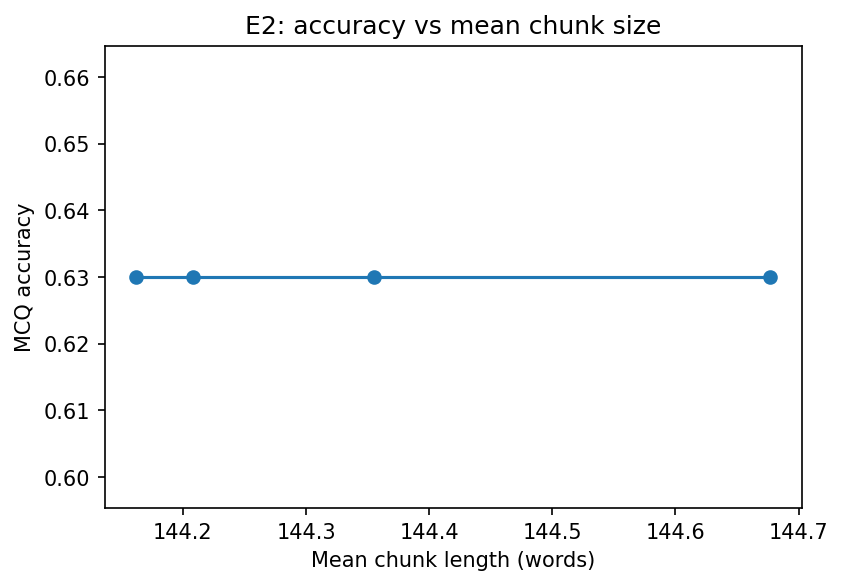
\includegraphics[width=0.82\linewidth]{e2_accuracy_vs_chunksize.png}
  \caption{\textbf{(E2)} MCQ accuracy versus mean chunk length proxy from the segmented corpus. The plotted relationship is visually flat.}
  \label{fig:e2}
\end{figure}

\begin{figure}[t]
  \centering
  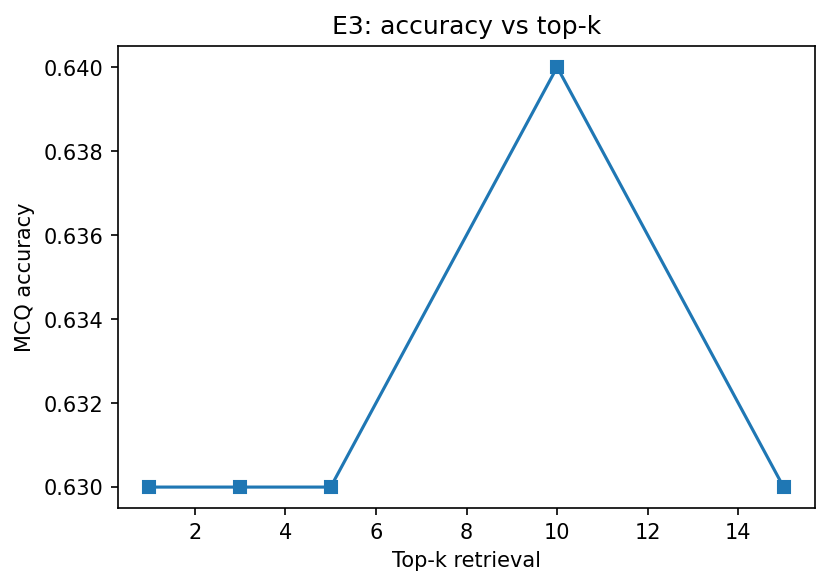
\includegraphics[width=0.82\linewidth]{e3_accuracy_vs_k.png}
  \caption{\textbf{(E3)} MCQ accuracy as a function of nominal top-\(k\). Variance across conditions is confined to \(\pm 0.005\) accuracy units on a 100-item test.}
  \label{fig:e3acc}
\end{figure}

\begin{figure}[t]
  \centering
  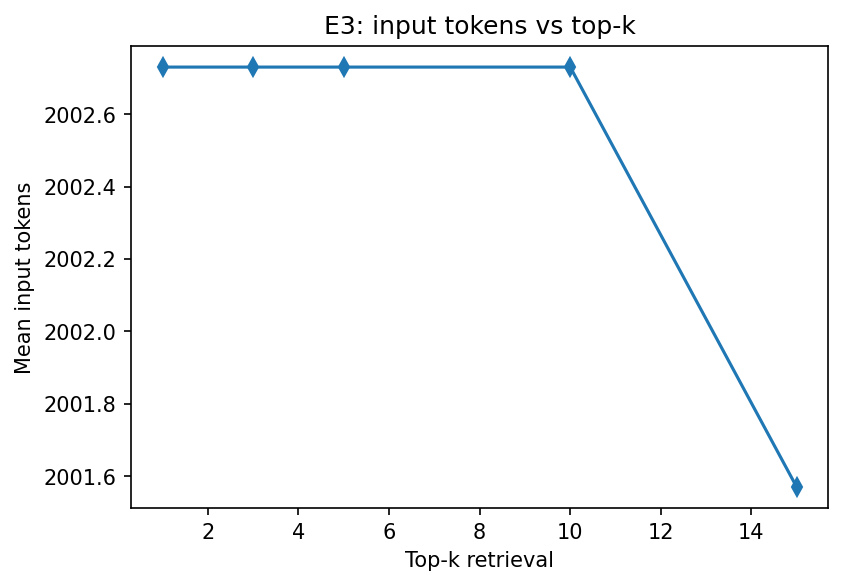
\includegraphics[width=0.82\linewidth]{e3_input_tokens_vs_k.png}
  \caption{\textbf{(E3)} Mean billed generator input tokens versus nominal \(k\). Plateau-shaped curve is indicative of pruning by similarity threshold before prompt assembly.}
  \label{fig:e3tok}
\end{figure}

\section{Discussion}
Three patterns deserve emphasis.

First, the \emph{chunk ceiling} ablation yielded \emph{no measurable change} under this particular segmentation policy and guideline mix. Interpretive caution is mandatory: equivalence is neither proven statistically nor implied beyond the factorial grid sampled. A plausible substantive story is that most clinically relevant retrieves already lived inside comparatively short sections bounded by headings, so widening the heuristic token budget rarely merged unrelated material.

Second, the \emph{naive} slicing baseline slightly \emph{outperformed} structure-aware segmentation in expectation, albeit without significance. Potential explanations include (i) stochastic coupling between PDF extraction artefacts and slicing boundaries,(ii) the MCQ probe being tolerant to heterogeneous context as long as a needle sentence appears anywhere in the fused prompt, or (iii) limited statistical power (\(n=100\), discordant pairs \(=4\)). Any claim of superiority of naive slicing would thus be overstated absent replication and significance.

Third, the \emph{top-\(k\) sweep} interacted with retrieval \emph{gating}: near-constant billed prompt lengths across \(k\) strongly suggest redundant nominal depth---extra neighbors below the similarity floor seldom reached the LM. Accuracy therefore stayed flat absent a substantive change to thresholding or embeddings. Operational latency regressions appear mostly mild except the \(k=1\) anomaly, underscoring interpreting latency traces from cloud APIs gently.

\textbf{Threats to validity}: single LM family; single stratified shard of AfriMed-QA; greedy decoding; correctness-only metric devoid of clinician-facing groundedness judgments; reproducibility hinges on uncontrollable API-side updates absent model pinning.

\section{Conclusions}
Within the confines of \(n{=}100\) MCQs on this guideline bundle, chunked dense RAG exhibited \emph{robust marginal insensitivity} to the swept chunk ceilings and retrieval depths tested, whereas structure-aware vs.\ naive preprocessing produced no decisive advantage despite mild directional surprise in point estimates.

Practically: defaulting structure-aware preprocessing remains reasonable for qualitative interpretability (coherent excerpts, attributable sections) even absent MCQ lift. Researchers repeating this study should (i) log and report similarity thresholds jointly with nominal \(k\), (ii) consider expanding \(n\) or analyzing item-level residuals, (iii) register whether decoder access is archived for fixed-version replication.

\section*{Hyperparameter blanks (fill prior to submission)}
\begin{itemize}
\item Decoder model identifier and embedding model identifier as reported by the provider.
\item Numerical similarity cutoff \(\tau\) applied when filtering retrieved passages.
\item Decoding temperature and cap on completion tokens for MCQ responses.
\item Whether provider model versions were pinned for replication.
\end{itemize}

\end{document}
